\section{Tutorial -- Flowsheet Result Data}\label{tutorials.fs.data}

Flowsheet evaluation results are stored in a table in the FOQUS session. This data can be used for many purposes.  The flowsheet evaluations may be single runs, part of an optimization problem, or part of a UQ ensemble. This tutorial provide information about sorting, filtering, and exporting data.

Copy the Data\bs Simple\_flow.foqus file from the example files to a convenient location (see section \ref{tutorial.example.files}).  This file is similar to the one created in the tutorial Section \ref{tutorial.simple.flow}, but it has been run an additional 100 times using a UQ ensemble (see Chapter \ref{chpt.uq}).

\begin{enumerate}
	\item Open FOQUS.
	\item Open the Simple\_flow.foqus session from the example files.
	\item Click the \bu{Flowsheet} button from the Home window.
	\item Click \bu{Flowsheet Data} in the toolbar on the left side of the Home window (Figure \ref{fig.data.table1}).
\end{enumerate}

\begin{figure}[H]
	\begin{center}
		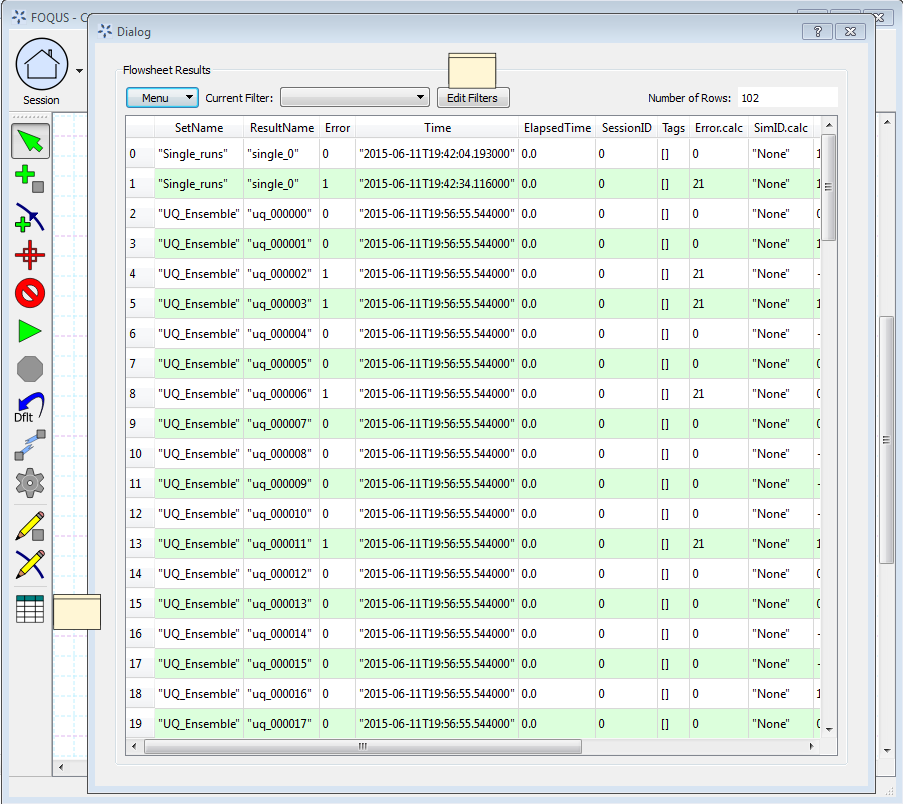
\includegraphics[scale=0.55]{Chapt_flowsheet/figs/data_table_1}
		\caption{Flowsheet Results Data Table, All Data}
		\label{fig.data.table1}
	\end{center}
\end{figure}

A data table should be displayed like the one shown in Figure \ref{fig.data.table1}.  There are 102 flowsheet evaluations.  The first two evaluations are single runs, as can be seen in the \textbf{\underline{SetName}} column, and the remaining 100 evaluation are from a UQ ensemble.  The \textbf{\underline{Error}} column shows several of the evaluations resulted in an error from a negative number being passed to the square root function.

This tutorial is broken up into mini-tutorials in the remaining subsections, which can be done independently.  They each use the example data file described above.

\subsection{Sorting Data}

\begin{enumerate}
	\item Open FOQUS.
	\item Open the Simple\_flow.foqus session from the example files.
	\item Click \bu{Flowsheet} in the main toolbar at the top of the FOQUS Home window.
	\item Click \bu{Flowsheet Data} in the toolbar on the left side of the Home window (Figure \ref{fig.data.table1}).
	\item Click \bu{Edit Filters} (Figure \ref{fig.data.table1}).
	\item Click \bu{New Filter}.
	\item Enter ``Sort1'' as the new filter name.
	\item Click \bu{New Filter}.
	\item Enter ``Sort2'' as the new filter name.
	\item Select ``Sort1'' from the \bu{Filter} drop-down list.
	\item Select the \bu{Sort Data} checkbox.
	\item Enter \verb|["-result"]| as the \textbf{Sort Term\underline{}}. Include the square brackets. The square brackets indicate that there is a list of sort terms, although in this case there is only one. If multiple search terms are given, the additional terms will be used to sort results having the same value for the previous terms. The ``-'' in front of \textbf{\underline{result}} indicates the results should be sorted in reverse.  The names of the sort terms come from the column headings, and are case sensitive.
	\item Click \bu{Done} to save the filters and return to the results table.
\end{enumerate}

\begin{figure}[H]
	\begin{center}
		\includegraphics[scale=0.55]{Chapt_flowsheet/figs/filter_1}
		\caption{Sort1 Data Filter}
		\label{fig.filter.1}
	\end{center}
\end{figure}

\begin{enumerate}
	\setcounter{enumi}{13}
	\item Select ``Sort1'' from the \bu{Current Filter} drop-down list (Figure \ref{fig.filter.1.result}).
	\item The results are shown in Figure \ref{fig.filter.1.result}. The data should be sorted in reverse alphabetical order by \textbf{\underline{result}}. Some of the columns are hidden to make the relevant results easier to see.
\end{enumerate}

\begin{figure}[H]
	\begin{center}
		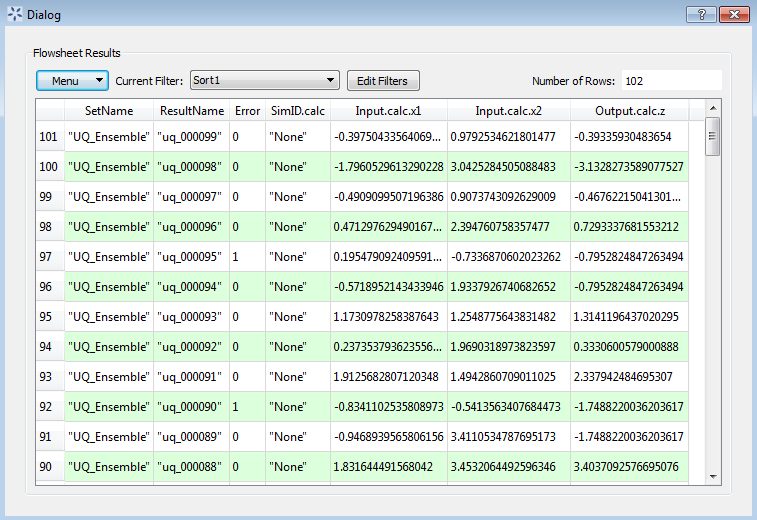
\includegraphics[scale=0.55]{Chapt_flowsheet/figs/filter_1_result}
		\caption{Sort1 Data Filter Results}
		\label{fig.filter.1.result}
	\end{center}
\end{figure}

\begin{enumerate}
	\setcounter{enumi}{15}
	\item Click \bu{Edit Filters} (Figure \ref{fig.filter.1.result}). The dialog box in Figure \ref{fig.filter.2} should display.
	\item Select ``Sort2'' from \bu{Filter} drop-down list.
	\item Select the ``Sort Data'' checkbox.
	\item Enter \verb|["Error", "-result"]| in the \bu{Sort Term} field.  This will sort the data first by \textbf{\underline{Error}} code then by \textbf{\underline{result}} in reverse alphabetical order.
	\item Click \bu{Done}.
\end{enumerate}

\begin{figure}[H]
	\begin{center}
		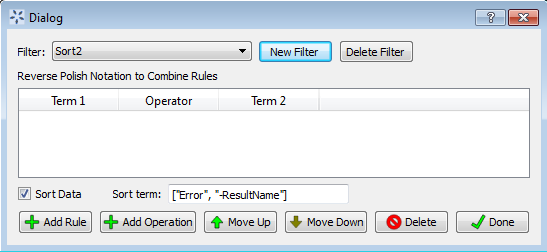
\includegraphics[scale=0.55]{Chapt_flowsheet/figs/filter_2}
		\caption{Sort2 Data Filter}
		\label{fig.filter.2}
	\end{center}
\end{figure}

\begin{enumerate}
	\setcounter{enumi}{20}
	\item Select ``Sort2'' in the \bu{Current Filter} drop-down list (Figure \ref{fig.filter.2.result}). 
	\item The results are shown in Figure \ref{fig.filter.2.result}. The data should be sorted so all \textbf{\underline{Error}} code zero results are first then sorted in reverse alphabetical order by \textbf{\underline{result}}.
\end{enumerate}

\begin{figure}[H]
	\begin{center}
		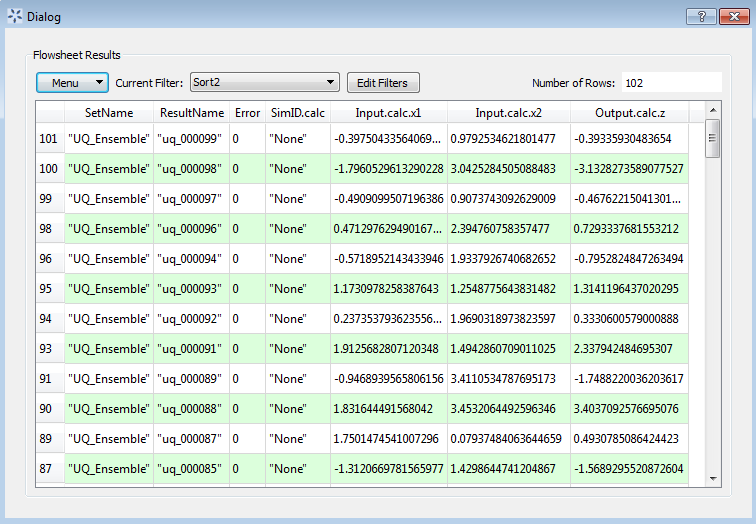
\includegraphics[scale=0.55]{Chapt_flowsheet/figs/filter_2_result}
		\caption{Sort2 Data Filter Result}
		\label{fig.filter.2.result}
	\end{center}
\end{figure}

\subsection{Filtering Data}

\begin{enumerate}
	\item Open FOQUS.
	\item Open the Simple\_flow.foqus session from the example files.
	\item Click the \bu{Flowsheet} button in the Home window.
	\item Click the Results Data button (Table icon in left toolbar).
	\item In the data table dialog, click \bu{Edit Filters}.
	\item Click \bu{New Filter} and enter ``Filter1'' in the \textbf{\underline{Filter}} field as the new filter name.
\end{enumerate}

The completed filter settings are shown in Figure \ref{fig.filter.3}. The buttons along the bottom of the filter editor dialog are used to add, delete, and change the order of rules and operations. Rules are conditions that are placed on data to be displayed. Operations are used to modify or combine rules. FOQUS uses reverse polish notation for the order of operations. The example filter in \ref{fig.filter.3} is equivalent to (Error = 0 AND SetName $\in$ \{UQ\_Ensemble, Single\_runs\}) OR Index $<$ 3.

The filter terms can be numbers, strings, lists of numbers, lists of strings or column headings. When entering column headings as search terms, do not enclose the column heading in quotes. This distinguishes column heading names from strings. The other types of terms are in JSON format. Strings are enclosed in double quotes, numbers have no quotes, and lists are enclosed in square brackets with elements separated by commas. 

\begin{enumerate}
	\setcounter{enumi}{6}
	\item Click \bu{Add Rule} three times.
	\item Click \bu{Add Operation} two times.
	\item Fill out the rule and operation rows as shown in Figure \ref{fig.filter.3}.
	\item Click \bu{Done}.
\end{enumerate}

\begin{figure}[H]
	\begin{center}
		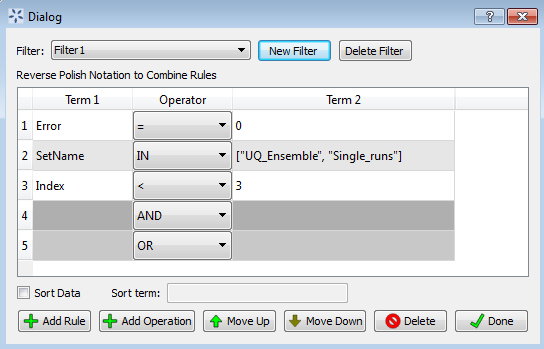
\includegraphics[scale=0.55]{Chapt_flowsheet/figs/filter_3}
		\caption{Filter1 Data Filter}
		\label{fig.filter.3}
	\end{center}
\end{figure}

\begin{enumerate}
	\setcounter{enumi}{10}
	\item In the data table dialog, select ``Filter1'' from the \bu{Current Filter} drop-down list.
	\item The result is displayed in Figure \ref{fig.filter.3.result}.
\end{enumerate}

\begin{figure}[H]
	\begin{center}
		\includegraphics[scale=0.55]{Chapt_flowsheet/figs/filter_3_result}
		\caption{Filter1 Data Filter Result}
		\label{fig.filter.3.result}
	\end{center}
\end{figure}

\subsection{Exporting Data}

This tutorial uses a spreadsheet program such as Excel or Open Office. The exported data is subject to the selected filter. See the previous tutorials in this section for more information about sorting and filtering data to be exported.

\subsubsection{Clipboard}

FOQUS can export data directly to the Clipboard. The data can be pasted into a spreadsheet or as text. Copying data to the Clipboard eliminates the need for an intermediate file when creating spreadsheets.

\begin{enumerate}
 	\item Open FOQUS.
 	\item Open a spreadsheet program.
 	\item Open the Simple\_flow.foqus session from the example files.
 	\item Click the \bu{Flowsheet} button in the Home window.
 	\item Click the Results Data button (Table icon in left toolbar).
 	\item Click on the \bu{Menu} drop-down list in the data table dialog.
 	\item Select ``Export'' from the \textbf{\underline{Menu}} drop-down list.
 	\item Click \bu{Copy Data to Clipboard}.
 	\item Select Paste in the spreadsheet program. The data table in FOQUS should paste into the spreadsheet. Filters can be used to sort or reduce the exported data.
\end{enumerate}

\subsubsection{CSV File}

CSV (comma separated value) files can be read by almost any spreadsheet program, and are common formats readable by many types of software. FOQUS exports CSV files using the column headings from the data table as a header.

\begin{enumerate}
 	\item Open FOQUS.
 	\item Open a spreadsheet program.
 	\item Open the Simple\_flow.foqus session from the example files.
 	\item Click the \bu{Flowsheet} button in the Home window.
 	\item Click the Results Data button (Table icon in left toolbar).
 	\item Click the \bu{Menu} drop-down list.
 	\item Select ``Export'' from the \textbf{\underline{Menu}} drop-down list.
 	\item Click \bu{Export to CSV File}.
 	\item Enter a file name in the file dialog.
 	\item In the spreadsheet program, open the CSV file exported in the previous step.
\end{enumerate}
